\documentclass[12pt,a4paper]{article}
\usepackage[utf8]{inputenc}
\usepackage[french]{babel}
\usepackage[T1]{fontenc}
\usepackage{amsmath}
\usepackage{amsfonts}
\usepackage{amssymb}
\usepackage{graphicx}
\usepackage{url}
\author{\textsc{TRAN Quoc Nhat Han} - \textsc{AMINE MOUSTATIH}}
\title{Recherche documentaire de tests d'adéquation}
\date{\today}
\begin{document}
\maketitle 
\renewcommand{\contentsname}{Sommaire}
\tableofcontents

\clearpage

\begin{abstract}
Ce rapport est un petit recherche documentaire concernant quelques tests d'adéquation usuels:
\begin{itemize}
\item Test $\chi^2$
\item Test de Shapiro-Wilk
\item Test d'Anderson Darling
\end{itemize}
\end{abstract}

\clearpage

\section{Test $\chi^2$}

\section{Test de Shapiro-Wilk}

\subsection{Histoire en bref}
Ce test non-paramétrique est publié en 1965 par \emph{Samuel Sanford Shapiro} et \emph{Martin Wilk} pour tester si un échantillon d'une variable \textbf{continue} (sous 2000 observations) suit \textbf{une loi normale}.

\subsection{Processus}

Soit une variable continue $X$ dont $n$ observations étaient réalisées $x_1, x_2, ..., x_n$.

Soient 2 hypothèses: 
\begin{itemize}
\item $H_0$: $X$ suit une loi normale $N(\mu, \sigma^2)$.
\item $H_1$: $X$ ne suit pas la loi normale.
\end{itemize}

Nous effectuons le test comme suivant:
\begin{enumerate}
\item Ordonner les réalisations dans l'ordre croissant $y_1 \leq y_2 \leq ... \leq y_n$.
\item Calculer \[{S^2} = \sum\limits_1^n {{{\left( {{y_i} - \overline y } \right)}^2}}  = \sum\limits_1^n {{{\left( {{x_i} - \overline x } \right)}^2}} \]
Donc $\overline y, \overline x$ désignent la moyenne de $y, x$ respectivement.
\item Calculer des différences (entre le premier $y_1$ et le dernier $y_n$, le deuxième $y_2$ et l'avant-dernier $y_{n-1}$, et ainsi la suite, le médian $y_{k+1}$ est ignoré si $n=2k+1$). Appliquer un coefficient de pondérer lu dans la table \ref{ShapiroWilkTablePonderer}. Les additionner et élever au carré.
\[{b^2} = {\left( {\sum\limits_1^{\left\lfloor {\frac{n}{2}} \right\rfloor } {{a_i}\left( {{y_{n + 1 - i}} - {y_i}} \right)} } \right)^2}\]
\begin{figure}[!h]
\centering
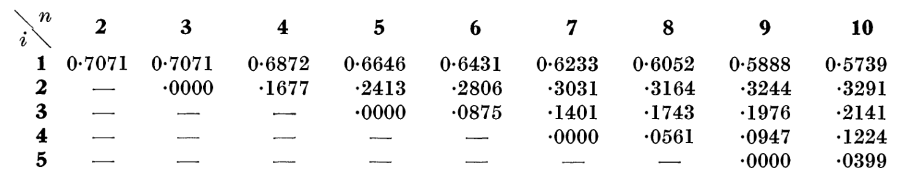
\includegraphics[width=\textwidth]{images/ShapiroWilk_N_1_10.png}
\caption{Coefficients $a_{n+1-i}$ pour $n=1..10$}
\label{ShapiroWilkTablePonderer}
\end{figure}
\item Calculer le statistique du test \[W = \frac{{{b^2}}}{{{S^2}}}\]
\item Rechercher la valeur $W$ dans la table \ref{ShapiroWilkTablePourcentage}. Petit $W$ signifie une distribution non normale.
\begin{figure}[!h]
\centering
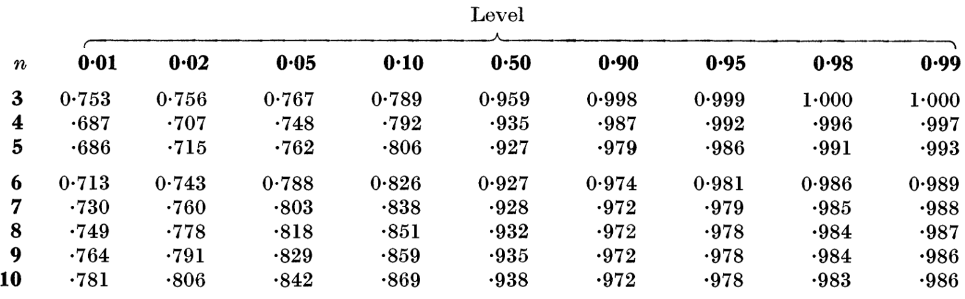
\includegraphics[width=\textwidth]{images/ShapiroWilk_Percentage.png}
\caption{Pourcentage de $W$ pour $n=1..10$}
\label{ShapiroWilkTablePourcentage}
\end{figure}
Choisir la valeur plus proche à $W$ dans la ligne correspondant à $n$. Regarder alors le niveau (\emph{level}) de signifiance $p-value$. Si $p-value > \alpha$ ($\alpha$ est le risque, souvent $1\%$ ou $5\%$), l'hypothèse $H_0$ est accepté.
\end{enumerate}
\subsection{Code en R}
\begin{verbatim}
shapiro.test(x)
\end{verbatim}

$x$ désigne un vecteur de données.

\subsubsection*{Exemples}
\begin{verbatim}
> shapiro.test(rnorm(100, mean = 5, sd = 3))

Résultat de la commande:

Shapiro-Wilk normality test

data: rnorm(100, mean = 5, sd = 3)
W = 0.9895, p-value = 0.6211
\end{verbatim}

$p$ est significativement plus grand que $\alpha=5\%$. L'hypothèse nulle est donc non rejetable.

\begin{verbatim}
> shapiro.test(runif(100, min = 2, max = 4))

Résultat de la commande:
Shapiro-Wilk normality test

data: runif(100, min = 2, max = 4)
W = 0.9337, p-value = 8.077e-05
\end{verbatim}

$p$ est trop faible. L'échantillon, par conséquence, ne suit pas la loi normale.
\section{Anderson Darling}

\clearpage

\begin{thebibliography}{3}
\bibitem{ShapiroWilk}

S. S. Shapiro et M. B. Wilk, An analysis of variance test for normality (complete samples)

\url{https://github.com/haghish/ST516/blob/master/Articles/Shapiro-Wilks%20test/An%20analysis%20of%20variance%20test%20for%20normality%20(complete%20samples).pdf}

\bibitem{TestsNormalite} 
\url{http://www.jybaudot.fr/Inferentielle/testsnormalite.html}

\bibitem{ShapiroWilkR}
\url{http://www.sthda.com/french/wiki/test-de-normalite-avec-r-test-de-shapiro-wilk}

\bibitem{ShapiroWilkRex}
\url{https://stat.ethz.ch/R-manual/R-patched/library/stats/html/shapiro.test.html}
\end{thebibliography}
\end{document}